
\chapter{Curva PWM x RPM}

\section{Não linearidade}

Depois de definido como calcular a velocidade o prózimo desafio foi lidar com a não linearidade entre o PWM e o resultado medido em RPM.

\begin{figure}[h]
	\centering
	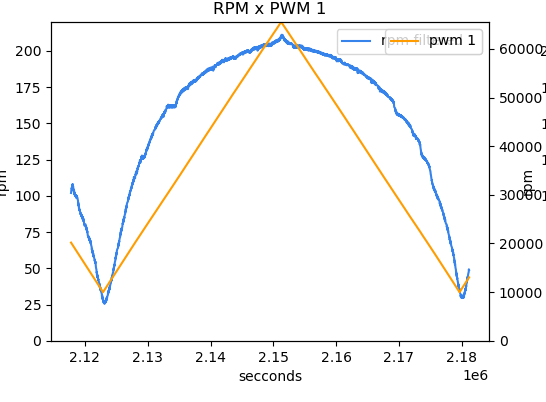
\includegraphics{figures/pwm_x_rpm}
	\caption{Curva PWM e RPM no tempo}
	\label{lof}
\end{figure}

Considerando essa não linearidade, foram realizadas 15k medições em PWM vs RPM para definir uma equação que pudesse relacionar o PWM com o RPM.


\begin{figure}[h]
	\centering
	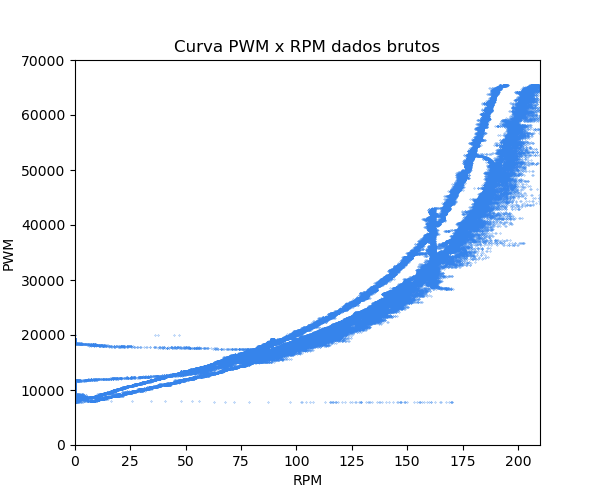
\includegraphics{figures/curva_pwm_x_rpm_dados_brutos}
	\caption{Curva PWM x RPM dados brutos}
	\label{lof}
\end{figure}


Limpeza dos dados realizada no python
\lstset{language=Python}
\begin{lstlisting}
    import json
    import pandas as pd
    import numpy as np
    import matplotlib.pyplot as plt
    
    res = open('mediadas_capturadas.txt').read()
    res = res.split('\n')
    
    res = [json.loads(i[i.find('''{"millis":'''):]) for i in res]
    
    dados_brutos = pd.DataFrame(res)
    
    dados_brutos = pd.concat([
        dados_brutos[['w1','filterRpm_1']]
        .rename(columns={'filterRpm_1':'filter_rpm_','w1':'w'}),
        dados_brutos[['w2','filterRpm_2']]
        .rename(columns={'filterRpm_2':'filter_rpm_','w2':'w'}),
        dados_brutos[['w3','filterRpm_3']]
        .rename(columns={'filterRpm_3':'filter_rpm_','w3':'w'})
    ]).sort_values('w')
    
    
    dados_medios = dados_brutos.groupby('w').agg({
        'filter_rpm_':['mean']
    }).reset_index()
    
    
    dados_medios.columns = [''.join(i) for i in dados_medios.columns]
    
    dados_medios['cut'] = (dados_medios['w']/200).astype(int)
    dados_medios_amostra = dados_medios.groupby('cut').first().reset_index()
    
    dados_medios_amostra[
        ['filter_rpm_mean', 'w']
    ].to_csv('amostra_invertida.csv', index=False)

\end{lstlisting}


\begin{figure}[h]
	\centering
	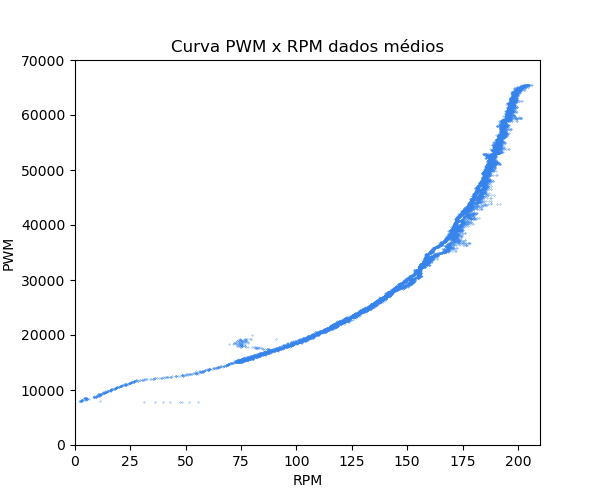
\includegraphics{figures/curva_pwm_x_rpm_dados_medios}
	\caption{Curva PWM x RPM dados médios}
	\label{lof}
\end{figure}


Matlab
\lstset{language=Matlab}
\begin{lstlisting}
    T = readtable('amostra_invertida.csv');
    filter_rpm_mean =  T{:,1};
    w =  T{:,2};
    f=fit(filter_rpm_mean,w,'poly4')

    f = 
    
         Linear model Poly4:
         f(x) = p1*x^4 + p2*x^3 + p3*x^2 + p4*x + p5
         Coefficients (with 0.95 confidence bounds):
           p1 =   0.0001131  (9.732e-05, 0.0001288)
           p2 =    -0.03064  (-0.0375, -0.02377)
           p3 =       2.993  (1.999, 3.988)
           p4 =      -1.257  (-54.15, 51.63)
           p5 =        9017  (8235, 9798)

\end{lstlisting}

\begin{figure}[h]
	\centering
	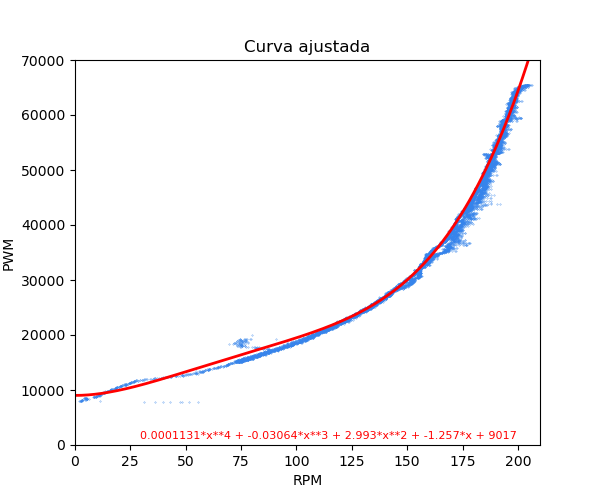
\includegraphics{figures/curva_ajustada}
	\caption{Curva ajustada}
	\label{lof}
\end{figure}


Polinônio da curva

\begin{equation}
    \begin{split}
        0.0001131x^{4} + -0.03064x^{3} + 2.993x^{2} + -1.257x + 9017
    \end{split}
\end{equation}

